\documentclass{standalone}
\usepackage[svgnames]{xcolor} % Enables a wide range of color names
\usepackage{tikz}
\usetikzlibrary{arrows,automata,positioning,shapes}
\usepackage{amsmath,amssymb,amsfonts}

\begin{document}
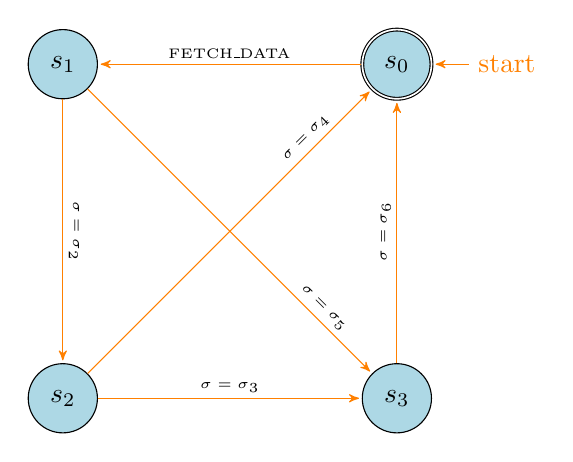
\begin{tikzpicture}[>=stealth',
                    shorten > = 1pt,
                    node distance = 1cm and 2cm,
                    el/.style = {inner sep=2pt, align=left, sloped, color=black, font=\tiny},
                    every label/.append style = {font=\tiny},
                    every node/.append style ={font=\normalsize},
                    every state/.append style={fill=LightBlue},
                    every edge/.append style={color=orange},
                    square/.style={regular polygon, regular polygon sides=4, minimum size=6cm, outer sep=0pt}
                    ]
\tikzset{
  sigma_1/.style={node contents=FETCH\_DATA},
  nameIP2/.style={node contents=192.168.0.1},
}

\node[square] (A) {};

\node[state,accepting,
      initial right] (q0) at (A.corner 1) {$s_0$};
\node[state]         (q1) at (A.corner 2) {$s_1$};
\node[state]         (q2) at (A.corner 3) {$s_2$};
\node[state]         (q3) at (A.corner 4) {$s_3$};

\path[->]
    (q0)  edge  node[el,above,sigma_1]   {}       (q1)
    (q1)  edge  node[el,above]  {$\sigma=\sigma_2$}        (q2)
    (q3)  edge  node[el,above]  {$\sigma=\sigma_6$}        (q0)
    (q2)  edge  node[el,above,pos=0.8] {$\sigma=\sigma_4$} (q0)
    (q1)  edge  node[el,above,pos=0.8] {$\sigma=\sigma_5$} (q3)
    (q2)  edge  node[el,above]  {$\sigma=\sigma_3$}        (q3);
\end{tikzpicture}
\end{document}